\ylDisplay
{The Sand buggy and Abra}% Problem name
{2021}% Year
{theory}% Round (mcq, theory, experiment)
{2}% Problem nr.
{physics}% Subject (physics, chemistry, biology)
{}% Difficulty (1-3)
{
% Syl:
\ifStatement
\subpart[The sand buggy]
A sand buggy (shown in Figure 1) is a vehicle that is used for transportation in deserts. Consider a sand buggy travelling with a constant speed of \SI{72.0}{\km\per\hour} climbing a sand dune which is shown as an inclined plane with an angle of inclination of 300. The sand buggy is dragging a box of mass 200 kg upwards. The opposition to motion of the box offered by the sand is \num{0.15} of the normal force exerted on the box by the sand.
\begin{figure}[!htbp]
  \centering
  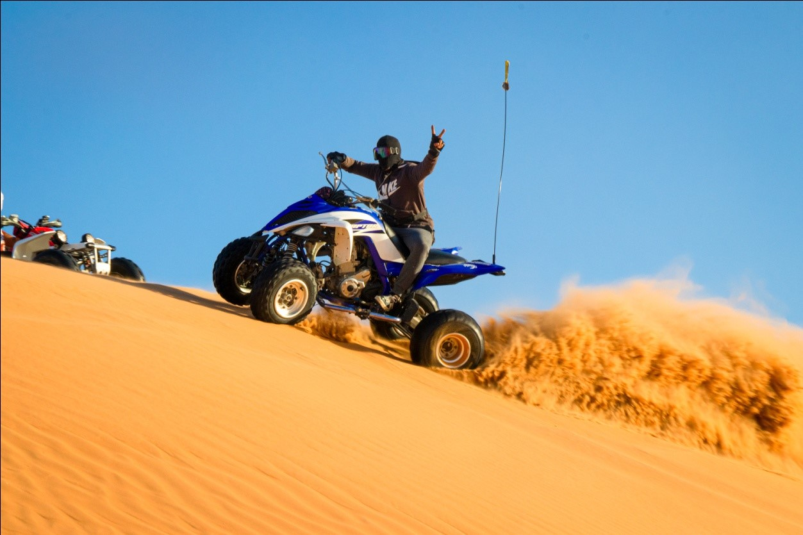
\includegraphics[width=0.7\linewidth]{2021-t-02-p1}
  \caption{Representative figure for sand buggy on a slope.}
\end{figure}

\prob
Draw a vector diagram showing all forces acting on the box in the figure below.
\begin{center}
  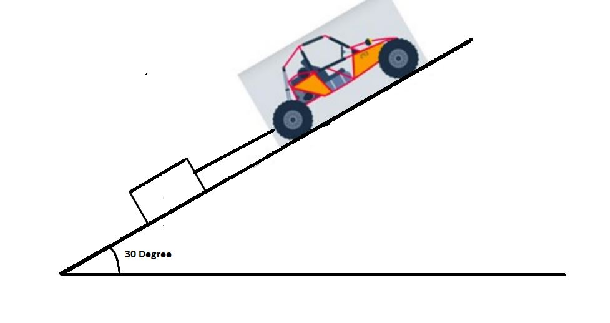
\includegraphics[width=0.5\linewidth]{2021-t-02-p2}
\end{center}

\prob
Calculate the total force (numerical value with proper unit) that opposes the motion of the box up the incline.

\prob
Calculate the minimum power (numerical value in SI unit) exerted by the sand buggy on the box to sustain the upward motion.

\prob
If the box is suddenly detached in the course of upward motion, calculate the retardation acting on the box.( Numerical value in SI unit)

\prob
How far will the box travel (numerical value in SI unit) before coming to rest after it detached from the sand buggy?


\subpart[Abra boat ride]
Dubai city’s traditional mode of transport to cross the creek is Abra boat ride (see Figure 2). Abra ride is one of the most economical modes of transport which connects the Old Dubai to New Dubai.
\begin{figure}[!htbp]
  \centering
  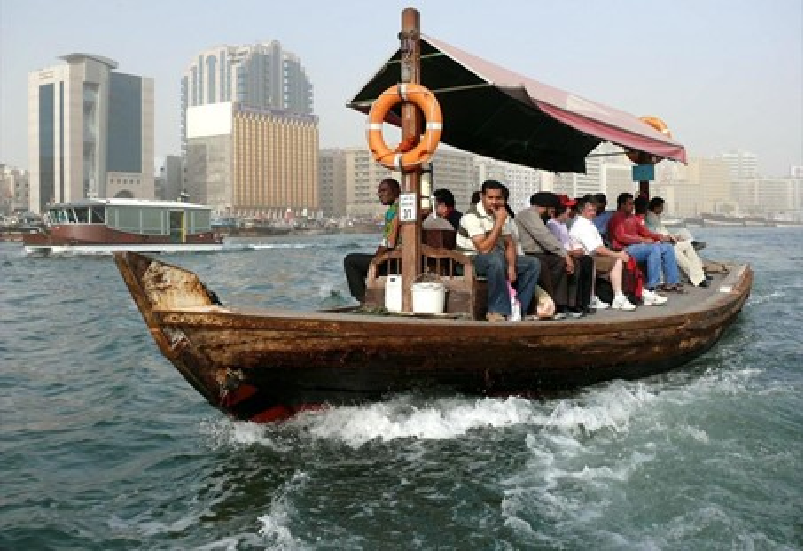
\includegraphics[width=0.7\linewidth]{2021-t-02-p3}
  \caption{Representative figure for Abra boat floating in water. }
\end{figure}

The boats are about 6 m in length and seating arrangement is made of two parallel lines of benches on either side of the vertical plane dividing the boat lengthwise. The centre of mass of the boat lies on the vertical line passing exactly through the centre of the benches. Passengers can seat on either side on the benches facing the creek.

When the passengers are seated, their centres of mass as a group can be considered to be at a height of \SI{0.4}{\m} above the deck. In case of a maximum payload the water level is \SI{0.5}{\m} below the deck, the buoyant force acts at a point \SI{0.1}{\m} below the water level and the centre of mass of the boat lies \SI{1.4}{\m} below the deck. The mass of the unloaded boat is 1000 kg while the average mass of each passenger is 65 kg.

Assume that the point of action buoyant force does not change considerably.

\prob
Draw a schematic sketch along the line $XY$, of the positions of centre of mass of the boat, centre of buoyancy of the boat, centre of mass of the passengers, and the deck level with respect to the water line and label the distances (need not be on scale). $CS$ represents the vertical cross section of the boat in the figure given below.
\begin{center}
  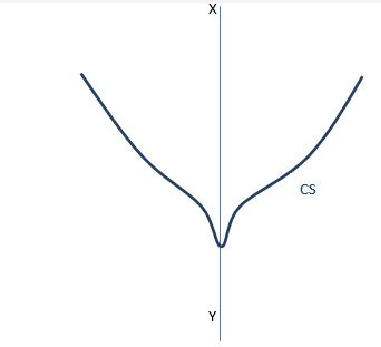
\includegraphics[width=0.5\linewidth]{2021-t-02-p4}
\end{center}

\prob
Calculate the maximum number of passengers can be seated such that the boat is prevented from capsizing.
\fi


\ifOption1

\fi


\ifOption2

\fi


\ifOption3

\fi


\ifOption4

\fi


\ifHint

\fi


\ifSolution

\fi


\ifEstStatement
% Problem name:

\fi


\ifEstOption1

\fi


\ifEstOption2

\fi


\ifEstOption3

\fi


\ifEstOption4

\fi


\ifEstHint

\fi


\ifEstSolution

\fi
}
